\documentclass[addpoints]{exam}

\usepackage{comment}
\usepackage{graphbox}
\usepackage{hyperref}
\usepackage{listings}
\usepackage{subcaption}
\usepackage{tabularx}
\usepackage{tikz}
\usetikzlibrary{positioning}

% Header and footer.
\pagestyle{headandfoot}
\runningheadrule
\runningfootrule
\runningheader{CS 440}{HW 2: Interactive WebGL}{Fall 2023}
\runningfooter{}{Page \thepage\ of \numpages}{}
\firstpageheader{}{}{}

\qformat{{\large\bf \thequestion. \thequestiontitle}\hfill[\totalpoints\ points]}
% \qformat{{\large\bf \thequestion. \thequestiontitle}\hfill}
\boxedpoints

\graphicspath{{images/}}

\title{Homework 2: Rendering with WebGL}
\author{CS 440 Computer Graphics\\Habib University}
\date{Fall 2023}

\begin{document}
\maketitle

Each problem below specifies the names of the files that you have to submit for it. Please make sure that your submitted files have the indicated names. Any files in your GitHub repository with these names at the time of the deadline will be considered your submission. Many of the problems refer to the {\tt map\_point} function from the previous homework.

We will use the utility files from \href{https://bit.ly/3Bqt8XG}{the website} of the newer edition of the textbook. Specifically, we will make use of the files containing ``ES6" in their names. These supersede similarly named files in the folder in that they are compliant with recent JavaScript (JS) standards which deprecate older features that are, in some cases, now considered insecure. In your HTML files, you may include the files, \texttt{MVES6.js} and \texttt{initShadersES6.js}, over the web, or you may include local copies.

GLSL has some helpful syntax and types to support geometric computation. You can read about them in the GLSL section toward the bottom of \href{https://webgl2fundamentals.org/webgl/lessons/webgl-shaders-and-glsl.html}{this page}.

\titledquestion{Essentials}
  \begin{parts}
  \part Go over \href{https://webgl2fundamentals.org/webgl/lessons/webgl-shaders-and-glsl.html#uniforms}{this page} for a quick recap on WebGL2 Shaders and GLSL. You may skip the sections on, ``Textures in Vertex Shaders''. and , ``Textures in Fragment Shaders''.
  \part Go over the page ``Including shaders from external files'' under the HW 2 module on Canvas. Make sure to understand and follow the instructions.
  \end{parts}
  


\begin{comment}
  \begin{itemize}
  \item Make colorabrs in different ways. Explain we will do it in many ways before ultimately doing it the right way.
    \begin{itemize}
    \item pass canvas width, W, as a uniform
    \item draw W vertical lines. (2W vertices) assign colors in verex shader, with menu choice for grayscale or colors
    \item make 2 triangles, do not send color, rather compute color for each fragment in fragment shader based on fragCoord
    \item make 2 triangles, assign color to vertices
    \item use above approach to render the colorbar with 6 or fewer vertices,
    \item [stretch] Draw both bars together using the above technique, either in different viewports in the same canvas, or on different canva on the same page.
    \end{itemize}
  \end{itemize}
\end{comment}

\begin{questions}

\titledquestion{Color Interpolation}[20]
  \label{q:colorbar}.
  
  \vspace{-30pt}
  \begin{center}
    \includegraphics[width=\linewidth]{barbw}\\
    \vspace{-75pt}\includegraphics[width=\linewidth]{barrgb}
  \end{center}
  \vspace{-50pt}\underline{Problem}: When drawing the \href{https://homepages.abdn.ac.uk/j.s.reid/pages/Maxwell/Legacy/MaxTri.html}{Maxwell triangle} in the recitation, we relied on the GPU's native color interpolation. We will now interpolate colors ourselves using {\tt map\_point}.

  \underline{Task}:
  \begin{parts}
  \part Display the colorbars above in your display window with the grayscale bar above the color bar. Each bar is comprised of vertical lines rendered next to each other, i.e. on adjacent pixels, in the display window. Both bars have the same dimensions. The width has to be sufficiently large to include every color in the following RGB ranges.
    \begin{itemize}
    \item (0,0,0) to (255, 255, 255), and
    \item (255,0,0) to (0, 255, 0) to (0, 0, 255).
    \end{itemize}
  \part Include mechanisms on your page to interactively change the colors that the bars interpolate between. The colorbars should update in response to changing the colors.
  \end{parts}
  \underline{Files}: colorbar.html, colorbar.js

\titledquestion{The Mandelbrot Set}[15]

  The sequence $z_n$ for a complex number, $c$, is defined for $n\geq 0$ as
  \[
    z_n(c) = \left\{
      \begin{array}{l@{\quad}l}
        0 & n = 0\\
        z^2_{n-1}(c)+c & \textrm{otherwise}
      \end{array}
    \right.
  \]

  \begin{figure}
    \centering
    \begin{tabular}{cc}
      \includegraphics[width=.47\linewidth]{mandelbrot1}& \includegraphics[width=.47\linewidth]{mandelbrot2}\\
      (a) & (b)
    \end{tabular}
    \caption{The Mandelbrot set up to $n_t = 100$. The points at the corners of the windows are outside the circle of radius 2, and $z_n$ escapes for these points at $n=1$. They are completely red. The points in blue toward the center of the image are the ones for which $z_n$ has not yet escaped. (a) Uniform color interpolation from Red to Green to Blue. (b) Adjusted color interpolation on the same data.}
    \label{fig:mandelbrot}
  \end{figure}
  
  The \href{http://en.wikipedia.org/wiki/Mandelbrot_set}{Mandelbrot set}, $M$, is the set of all complex numbers, $c$, for which $z_n(c)$ is \textit{bounded}, i.e. $|z_n|$ is finite for all $n$. It can be shown for a given $c$ that if $|z_{n}(c)| > 2$ for some $n = n_0$, then the sequence $z_n(c)$ {\it escapes to infinity}, i.e. $z_n(c)$ is not bounded for $n > n_0$. Thus, for $c\in M$, $|z_n(c)| \leq 2$ for all $n\geq 0$. Since $z_1(c) = c$, we also have that $|c| \leq 2$. Therefore, $c\in M$ implies that:
  \begin{enumerate}
  \item $|c|\leq 2$
  \item $\forall n\geq 0:\, |z_n(c)|\leq 2$
  \end{enumerate}
  Condition 1 implies that every $c\in M$ lies within the circle in the complex plane centered at the origin and with radius 2. The value of $n$ for which condition 2 becomes false for a given $c$ is dubbed the {\it escape time} of $c$.

  \underline{Example}: Consider the complex numbers and the corresponding sequence for each up to $z_5$ in Table \ref{tab:mandelbrot}.
  \begin{table}
  \[
    \begin{array}{c|*{4}{|c}}
      & c=(3+4j) & c=(1+1j) & c=(0.5+0.5j) & c=(-0.5-0.5j)\\\hline\hline
      z_0(c) & 0 & 0 & 0 & 0\\
      |z_0(c)| & 0 & 0 & 0 & 0\\\hline
      z_1(c) & (3+4j) & (1+1j) & (0.5+0.5j) & (-0.5-0.5j)\\
      |z_1(c)| & 5.0 & 1.41 & 0.71 & 0.71\\\hline
      z_2(c) &  & (1+3j) & (0.5+1j) & (-0.5+0j)\\
      |z_2(c)| &  & 3.16 & 1.12 & 0.5\\\hline
      z_3(c) &  &  & (-0.25+1.5j) & (-0.25-0.5j)\\
      |z_3(c)| &  &  & 1.52 & 0.56\\\hline
      z_4(c) &  &  & (-1.69-0.25j) & (-0.69-0.25j)\\
      |z_4(c)| &  &  & 1.71 & 0.73\\\hline
      z_5(c) &  &  & (3.29+1.34j) & (-0.09-0.16j)\\
      |z_5(c)| &  &  & 3.55 & 0.18\\\hline
    \end{array}
  \]
  \caption{Examples of $z(n), 0\leq n\leq 5$ for some values of $c$. The magnitude of each value of $z(n)$ is also shown.}
  \label{tab:mandelbrot}
\end{table}
\begin{itemize}
  \item We see that $z_1=c$. This follows from the definition of $z_n$.
  \item For the first number, $(3+4j)$, we see that $|z_1|>2$. We can therefore say that $z_n$ will escape to infinity and the escape time of $(3+4j)$ is 1. This is expected as $(3+4j)$ lies outside the circle at the origin with radius 2.
  \item The second number, $(1+1j)$, lies within the required circle. But it escapes at n=2.
  \item The escape time for the third number, which is also inside the circle, is 5.
  \item The fourth number is also inside the circle and has not escaped until n=5. It may escape later or it may not. We cannot say.
  \end{itemize}
  
  \underline{Problem}: We want to visualize the Mandelbrot set up to a certain value of $n=n_t$ in an image. We will map to our viewport the circle in the complex plane which is centered at the origin and has a radius of 2. This will yield the complex number corresponding to each pixel in the view port. We will color each pixel according to the escape time of its corresponding complex number. In Figure \ref{fig:mandelbrot}, complex numbers that escape early are assigned red and those that have not escaped till $n=n_t$ are assigned blue. Complex numbers with intermediate escape values are assigned interpolated colors.

  Various steps are involved.
  \begin{enumerate}
  \item Map the x extent of the viewport to $[-2,2]$ on the real axis in the complex plane.
  \item Map the y extent of the viewport to $[-2j,2j]$ on the imaginary axis in the complex plane.
  \item Find the escape time of the complex number corresponding to each pixel in the viewport.
  \item Compute a color for a given escape time.
  \end{enumerate}

  \underline{Task}:
  \begin{parts}
  \part Visualize the Mandelbrot set as described above with $n_t$ defined as a global variable at the beginning of your JS file. You will find that a simple linear interpolation between the colors for $n=1$ and $n=n_t$ will lead to a bland visualization as seen in Figure \ref{fig:mandelbrot}a). You are encouraged to think about and implement a more discriminating color scheme for the escape times. You may implement any coloring scheme that sufficiently distinguishes between different escape times.
  \part Include a mechanism on your page, e.g. a slider, to control the value of $n_t$ within a reasonable range. The render should update in response to changes in the value.
  \end{parts}
  \underline{Tips and Notes}:\\
  --\ As you may imagine, this computation can be expensive. Pick a range for $n_t$ that is feasible for your machine and leads to an interesting visualization.\\
  --\ Make liberal use of \texttt{map\_point}. Points 1, 2, and 4 above lend themselves simply to its use.\\
  --\ You are encouraged to use the \texttt{Complex} type from \texttt{math.js}. See its usage \href{https://mathjs.org/docs/datatypes/complex_numbers.html}{here}. To use it in your JS code, include the following line in your HTML file.\\
  \verb|<script src="https://unpkg.com/mathjs@9.5.0/lib/browser/math.js"></script>|

  \underline{Files}: mandelbrot-cpu.html, mandelbrot-cpu.js

  \titledquestion{Boundary and Interior}[15]

    \underline{Problem}: We are going to render a triangle along with its boundary edges. The triangle and its edges are colored independently.
    
    \underline{Task}: Render the (filled) triangle and its boundary as described above and include in your page, interactive controls for the following.
  \begin{itemize}
  \item Set the RGB colors of the boundary vertices.
  \item Set the RGB colors of the triangle (interior) vertices.
  \item Toggle the display of the boundary.
  \item Toggle the display of the triangle (the interior).
  \item Assign a random color to the boundary vertices.
  \item Assign a random color to the triangle vertices.
  \end{itemize}
  \underline{Files}: colors.html, colors.js
  
  \titledquestion{Subdivision: $\lim\limits_{n\rightarrow\infty} \diamond = \circ$}[20]
  \begin{center}
    \includegraphics[width=\linewidth]{circle}
  \end{center}

  \begin{tabularx}{\linewidth}{lX}

    \raisebox{-\totalheight}{
      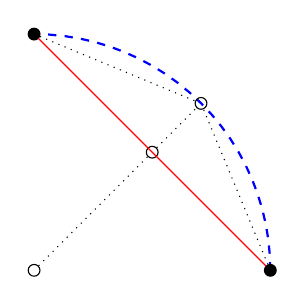
\begin{tikzpicture}
        \draw [blue,thick,dashed,domain=0:90] plot ({3*cos(\x)}, {3*sin(\x)});    
        node[circle,fill]{}(
        \node [draw,circle,fill,inner sep=1.5pt] at (0,3) (a){};
        \node [draw,circle,fill,inner sep=1.5pt] at (3,0) (b){};
        \node [draw,circle,inner sep=1.5pt] at (0,0) (c){};
        \node [draw,circle,inner sep=1.5pt] at (1.5,1.5) (p){};
        \node [draw,circle,inner sep=1.5pt] at (2.12,2.12) (q){};

        \draw [red] (a) -- (b);
        \draw [dotted] (c) -- (p);
        \draw [dotted] (p) -- (q);
        \draw [dotted] (a) -- (q);
        \draw [dotted] (b) -- (q);
      \end{tikzpicture}
    }
    &
      \underline{Problem}: For rendering purposes, a computer approximates a smooth shape with a many-sided polygon. We will approximate a circle with a successively refined diamond shape shown on the left in the figure above. Each successive shape in the figure is a refinement or \textit{subdivision} of the previous shape. The subdivision step inserts edge midpoints into the shape and projects them to the circumference of the circle being approximated. This is illustrated in the figure on the left. The red line approximates the blue arc. In the subdivision step, the midpoint of the red line is inserted and projected to the arc. The red line is then replaced with the dotted black lines.
  \end{tabularx}

    \underline{Task}:
    \begin{parts}
    \part Render a subdivided version of the diamond shown above.
    \part Include a mechanism to interactively alter the number of subdivision steps. The diamond corresponds to 0 steps, and each successive shape in the figure above represents one further subdivision.
    \end{parts}
    \underline{Files}: circle.html, circle.js

  
  \titledquestion{Koch Snowflake}

\begin{tabularx}{1.0\linewidth}{cX}
    \includegraphics[width=.3\textwidth,align=t]{koch1}
  &
    \vspace{10pt} \underline{Problem}: We will render a \href{https://en.wikipedia.org/wiki/Koch_snowflake}{Koch snowflake} which is a \href{http://mathworld.wolfram.com/Fractal.html}{fractal} generated by repeatedly applying a fixed transformation to all line segments. The figure on the left shows the starting shape on the top left and, proceeding left-to-right top-to-bottom, the result of successive applications of the transformation which is illustrated below.
    
    {\begin{tabularx}{0.63\textwidth}{cX}
    \includegraphics[scale=.7,align=t]{koch2}
      & The line segment $AB$ is replaced by the polyline $APQRB$ where the length of all shown line segments is equal to $\frac{|AB|}{3}$.
    \end{tabularx}}
\end{tabularx}

\underline{Task}:
\begin{parts}
\part Render the Koch snowflake at a desired recursion level.
\part Include a mechanism on your page to interactively alter the recursion level. The render should update according to the change in recursion level.
\end{parts}
    \underline{Files}: koch.html, koch.js
    

  
  \titledquestion{Sierpinski Triangle}[20]
  
  \begin{figure}
    \centering
    \begin{tabular}{cc}
      \includegraphics[width=.4\linewidth]{sierpinski}
      &
      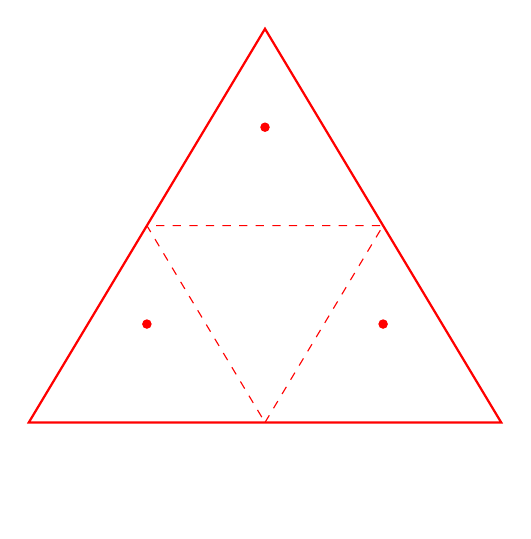
\begin{tikzpicture}
        \draw[red,thick] (0,0) -- (6,0) -- (3,5) -- cycle;
        \draw[red,dashed] (3,0) -- (4.5,2.5) -- (1.5,2.5) -- cycle;
        \draw[red,fill] (1.5, 1.25) circle (1.5pt);
        \draw[red,fill] (4.5, 1.25) circle (1.5pt);
        \draw[red,fill] (3, 3.75) circle (1.5pt);
        
        \node at (3,-1) {};
      \end{tikzpicture}\\
      (a) & (b)
    \end{tabular}
    \caption{(a) A Sierpinski triangle at recursion level 5. (b) The triangles that are subdivided in the recursive step in the generation of the Sierpinski triangle.}
    \label{fig:sierpinski}
  \end{figure}
  
\underline{Problem}: We will render the \href{https://en.wikipedia.org/wiki/Sierpinski_triangle}{Sierpinski triangle}, a \href{https://en.wikipedia.org/wiki/Self-similarity}{self-similar} geometric shape with many interesting properties, not the least of which is the variety of ways in which it can be generated. A sample triangle is shown in Figure \ref{fig:sierpinski}a).

We will generate the Sierpinski triangle recursively as illustrated in Figure \ref{fig:sierpinski}b). Starting with a triangle, connect all its edge midpoints. This yields 4 new triangles. Repeat the process for all the new triangles shown with a dot in them. Do not subdivide the triangle in the middle (without a dot). Note that the dots in the figure are for demonstration purposes only--they are not part of the Sierpinski triangle.

\underline{Task}:
\begin{parts}
\part Render the Sierpinski triangle as described above at any desired recursion level.\\
\part Include a mechanism on your page to interactively alter the recursion level. The render should update according to the change in recursion level.
\end{parts}
  \underline{Files}: sierpinski.html, sierpinski.js


  
\titledquestion{Mandelbrot on Shaders}[15]
  \underline{Problem}: We want to visualize the MAndelbrot set as before but perform color computation in the fragment shader, i.e. on the GPU, as opposed to the JS file, i.e. the CPU. As the calculation at each pixel of the visualization is completely independent of the other pixels, this task is perfectly suited for the fragment shader.

  There are several issues to tackle here.
  \begin{itemize}
  \item What data needs to be passed to the fragment shader: what information does the fragment shader need in order to compute the color.
  \item What data needs to be passed to the vertex shader: our program does not talk to the fragment shader, rather it can pass data to the vertex shader which can then pass data to the fragment shader.
  \item What attributes need to be passed to the vertex shader: the vertex shader runs once per vertex but vertices define a polygon which rasterizes to numerous pixels and the fragment shader runs for each pixel. The attributes passed to the vertex shader must be such that each rasterized pixel obtains a version of the data that is right for it.
  \item Many others.
  \end{itemize}
  Thinking about and finding solutions to these sub-problems is an intended part of this problem.
  
  \underline{Task}: Visualize the Mandelbrot set as in the earlier question but perform the color computation on the GPU.
  
  \underline{Files}: \texttt{mandelbrot-gpu.html, mandelbrot-gpu.js}

  
\titledquestion{Polygons Galore}[15]
  \label{q:galore}
  
  \begin{tabularx}{\linewidth}{lX}
    \includegraphics[width=.3\textwidth,align=t]{galore}
    &
      \vspace{20pt} \underline{Task}: We love polygons and cannot get enough of them. We will draw a limited set of polygons whose vertices are specified by the user through mouse clicks and are connected as per the current \textit{drawing mode}. For example, if \textit{triangle mode} is on, every 3 successive vertices will be connected to form a triangle.
  \end{tabularx}
  
  \underline{Task}: Interactively draw triangles and quadrilaterals based on vertices specified by mouse clicks in the canvas. Your program should support two drawing modes--triangle mode (default) and quad mode. Vertices that are not yet part of a polygon are drawn as points. Each drawn shape is assigned a different random color. Furthermore, the following interaction is supported.
  \begin{parts}
  \part Pressing \texttt{r} or \texttt{R} resets to default. That is, the canvas is cleared and the drawing mode is set to triangle mode.
  \part Pressing \texttt{t} or \texttt{T} toggles between the drawing modes. Vertices that have not yet completed a polygon at the time of the toggle should be handled according to the new mode, they should not be discarded. Polygons drawn before the toggle should not be affected.
  \end{parts}
  \underline{Files}: {\tt galore.html, galore.js}

\titledquestion{Tetrix}[15]

  \begin{tabular}{ccc}
    \includegraphics[width=.3\textwidth]{tetrix1}
    & \includegraphics[width=.3\textwidth]{tetrix2}
    & \includegraphics[width=.3\textwidth]{tetrix3}
  \end{tabular}

  \underline{Problem}: We will render a \href{http://mathworld.wolfram.com/Tetrix.html}{\it tetrix} which is the 3D version of the Sierpinski triangle and is also referred to as the \textit{Sierpinski tetrahedron}. Widgets on the page will control the rotation of the tetrix.

  When the visualization loads, the tetrix is rotating continuously about an arbitrary axis--$x, y,$ or $z$. 

  \underline{Task}:
  \begin{parts}
  \part Render the tetrix at any desired recursion level and rotating continuously about any axis.\\
  \part Include a mechanism on your page to interactively alter the recursion level. The rotation should remain unaffected. A recursion level of 0 corresponds to a completely filled tetrahedron. The left-most tetrix in the figure corresponds to a recursion level of 1.\\
  \part Include a mechanism on your page to interactively freeze and resume rotation.
  \part Include a mechanism on your page to interactively reset the tetrix to a default position.
  \part Include a mechanism on your page to interactively change the axis of rotation. 
  \end{parts}
  \underline{Files}: {\tt tetrix.html, tetrix.js}

\end{questions}

\end{document}

%%% Local Variables:
%%% mode: latex
%%% TeX-master: t
%%% End:
